\chapter{Overview of Machine Learning Technologies}
\label{chap: Chapter 3}
The development in Machine Learning and Information Retrieval in recent years resulted in a surge in recommender systems. However, machine learning and information retrieval plays a integral part in the success and failure of a recommender system. This chapter \ref{chap: Chapter 3} will cover the three popular types of learning: (1) reinforcement learning, (2) supervised learning, and (3) unsupervised learning. Followed by document cluster, how it works and challenges pertaining to document clustering. This chapter will investigate the different problems Natural Language Processing faces and what tasks are involved. Lastly, Topic Modelling will be discussed and how it was used.

\section{Machine Learning} \label{ssec:MLoverview}
Machine Learning (ML) is a subfield of Artificial Intelligence that is concerned with building algorithms which rely on a collection of some phenomenon \cite{Andriybook2019}. These examples can come from nature or, created by developers or, generated by other ML algorithms. Machine Learning is also known as attempting to solve problems by: (1) acquiring a dataset, and (2) automatically building a model using that dataset \cite{sebastiani2002machine}.
The rise of big data in recent years has created a problem of how to translate untouchable data into knowledge. The technological advances enabled Machine Learning to solve these problems. Machine Learning plays an integral part in the following sectors \cite{alpaydin2009introduction}:
\begin{itemize}
  \item Computational finance - in the credit section of banks, credit scoring.
  \item Computer vision - for face recognition, object detection and motion detection.
  \item Natural Language Processing - text analysis and text summarization.
\end{itemize}

Games or simulations were not mentioned in above mentioned list. Simulations brings forth a new need that has to be satisfied. Furthermore, simulation brings a decision making aspect.

\subsection{Reinforcement Learning}
Reinforcement Learning (RL) can be defined as an machine, capable of getting the state of an environment as input also known as features \cite{DBLP:journals/corr/abs-1806-08894}.
Actions are executed within each state. Furthermore, each action can give rewards which can move the machine to another state. As mentioned, Reinforcement Learning works on a reward system and each component like in figure \ref{fig:RLreward} will be discussed below.
\begin{figure}[htbp]
\centering
\includegraphics[width=6cm]{./figures/reinforce7.png}
\caption{Reinforcement Learning reward system \protect\cite{sebastiani2002machine}}
\label{fig:RLreward}
\end{figure}
\begin{itemize}
  \item Autonomous Agent: It is the agent's responsibility to take action.
  \item Actions: It can be seen as a set of logical steps which is needed to move forward. An action can be in two states, either reward or penalty.
  \item Environment: This is the environment in which the autonomous agent finds itself.
  \item Reward: The main aim of Reinforcement learning is to obtain rewards, good or bad.
  \item State: Is defined as the position it finds itself in the environment. To move around in the environment, the state needs to keep changing.
\end{itemize}
The goal of an reinforcement learning algorithm is to learn a near optimal policy, that thrives on the rewards system. A policy is the rules of the game. Reinforcement Learning focuses on addressing problems which includes decision making  \cite{Andriybook2019}. This works well for games, robotics and logistics.

\subsection{Supervised Learning}
Supervised Learning (SL) can be defined as a task that is learning the mapping between input and output by looking at examples of the input and output pairs. It creates a model from the labeled training data consisting of a set of training examples. By labeled, it suggests that the mapping between questions and answers, or between input and output has already been done \cite{singh2019natural}.
For example, if we look at a financial company that wants to look at users profiles to decide to give them a loan or not. A Machine Learning model would be trained on historical labeled data, which consists of information regarding profiles of the past customers \cite{kotsiantis2007supervised}.
The methodology that is used in Supervised Learning can sometimes vary based on the output of the model. Some supervised machine learning algorithms are listed here:
\begin{itemize}
  \item Logistic Regression
  \item Decision Trees
  \item Linear Regression
  \item Support Vector Machines
\end{itemize}

Another integral part of Supervised Learning is evaluating the model. Based on the type of model, shown above, the appropriate evaluation metric can be chosen and applied \cite{sebastiani2002machine}. Furthermore, this can be done by splitting the training data into two sets, train set, and validation set. Training of the model would be done on the training set and testing the performance should be done on the labeled validation set. Changes can be made in the Hyperparameters to improve the performance of the model \cite{kotsiantis2007supervised}. Hyperparameters are used to configure various aspects of the learning algorithm and does have a direct impact on the results and the performance of the created model. 

\subsection{Unsupervised Learning}
In Unsupervised Learning, a model is trained on similar unlabeled data. Since the data does not contain labels and sometimes unstructured, the model will just be trained without any influence given by labels. In Unsupervised Learning, the machine tries to find latent patterns and insights into the data that can be used in any form. The relevant Unsupervised Learning algorithms are:
\begin{itemize}
\item Clustering Algorithms (Document and Hierarchical)
\item Dimensionality Reduction Techniques
\item Topic Modeling
\end{itemize}

The rest of chapter \ref{chap: Chapter 3} will cover different applications of unsupervised learning, and how they interact with one another.

\section{Document Clustering}
Clustering is the answer to a problem of learning to map a label to examples based on an unlabeled dataset. Due to the dataset being unlabeled one must decide whether the learned model is optimal, which makes it much more complicated than Supervised Learning. Clustering has several use-cases ranging from text analysis to anomaly detection. A common use-case for businesses is to use machine learning driven clustering for profiling customers based on their activities and building strategies around these results. 

Search engines has been employing clustering by finding similar searches and results in one cluster. Document clustering, a branch of clustering, is the technique data mining uses which includes concepts from fields of Machine Learning, Information Retrieval and Natural Language Processing. Document clustering organizes documents into different groups called clusters, were the documents in the cluster share some common features according to the similarity measure. Clustering in general can produce overlapping clusters or non-overlapping clusters. In an overlapping cluster, it is likely multiple clusters can contain the same document \cite{andrews2007recent}, in a non-overlapping cluster, the opposite can happen. 

An example of supervised learning and unsupervised learning in terms of document clustering can be in document classification, all the classes and their properties are known beforehand. In document clustering, all the properties, or other information are unknown. Thus, classification is an example of supervised learning, and clustering is an example of unsupervised learning \cite{andrews2007recent}.

It can be defined that document clustering can be broken down into two sections, hard clustering, and soft clustering \cite{chen2010integration}. Furthermore, soft clustering can be broken down even more into partitioning and hierarchical.
\begin{itemize}
\item Hard: Clusters the features to exactly one cluster.
\item Soft: Clusters features into multiple clusters. For example: if the papers title needed to be clustered, named "Natural Language and Information Retrieval" would be clustered in both cluster names "Natural Language Processing" and "Information Retrieval".
\begin{itemize}
    \item Partitioning: This type of clustering splits the documents into fixed amount of clusters. An example is K-Means clustering \cite{chen2010integration}. 
    \item Hierarchical: Commonly known as taking shape as a tree of clusters.
  \end{itemize}
\end{itemize}
In this section, we discussed what document clustering is, talking about the different types of clustering. In the next section, the applications of document clustering will be discussed.
\subsection{Document Clustering Applications}
As mentioned above, document clustering falls within supervised learning and can be used in various fields like business and science \cite{jain2010data}. The origin of document clustering research was to improve recall or precision in Information Retrieval (IR) systems, however, recently the application of document clustering evolved drastically.  Document clustering can be applied for example \cite{jajoo2008document,abualigah2017text}:
Firstly, a system which enables people to find similar documents to that what was inputted. Using document clustering enabled systems to find other documents semantically similar \cite{Shah2013}. In recent years, the rate of development in technology spiked research on how to improve document clustering \cite{alhawarat2018revisiting,mekonnen2017topic}. 
Secondly, it is useful to organize large amount of documents in a taxonomy structure.
Thirdly, with the number of documents in the information ocean created a need to find duplicates. Clustering use-cases includes plagiarism detection, identifying related news stories and fake news, and to optimise search engines \cite{jin2016news}.
Lastly, in the most basic form, an academic is recommended papers based on the papers they have already read. This can be done by using clustering and employing other features of the text, and ultimately, improving the quality of recommendations. The use of Latent Dirichlet Allocation and content-based filtering is evident that it can work well as depicted in \cite{yeh2010}.

\subsection{Document Clustering Procedure}
Getting from a collection of documents to a cluster of documents a few processes needs to be followed. The processes comprises generally of three components: 1. feature extraction and selection, 2. document representation, and  3. document clustering \cite{shah2012document}.

Feature extraction takes the document and applies pre-processing steps to it. Cleaning the text includes removal of stop words which should be updated with the domains most common keywords, which would not add any value from a semantic perspective. The document should then be analysed and features should be extracted \cite{mugunthadevi2011survey}. Looking at the extracted features, selecting the right ones would be an important exercise to further remove noise. The benefit is that dimensionality is also reduced by only selecting the wanted features, it helps by enabling better data understanding \cite{wei2006combining}.

After the document has been stripped from all the unnecessary features, the documents are then only left with features which scored the highest in the metric score \cite{Shah2013}. Term Frequency (TF) would be an example of feature selection metrics. The documents are then grouped into clusters based on their features and metric scores which was calculated \cite{wei2006combining}.

\subsubsection{Term Frequency-Inverse Document Frequency (TF-IDF)}
The dataset that will be clustered will be represented as a set of vectors and the vector are called the vector of an object. Vector Space Model (VSM) is an model that represents text documents as vectors \cite{clark2015vector}. 

Term weight value can be defined as the noteworthiness of a specific term in a document. This can be calculated by the number of times the term is occurring within the document over the entire dataset. Term Frequency with Inverse Document Frequency (TF-IDF) is the most commonly used term weight scheme  \cite{cui2005document}. More frequent the words in a document the more important \cite{peng2006recent}.

\subsubsection{Dimension Reduction}

The increase in vast amounts of data has highlighted the inefficiency of most dimension reduction algorithms \cite{mugunthadevi2011survey}. These algorithms are used for feature extraction and feature selection. While feature extraction is taking place, new features are combined with the original features, which causes computation load to increase. In contrast to feature extraction,  feature selection selects the features directly.

\subsection{Similarity Measures for Document Clustering} \label{JSD}

Cluster similarity are based on the measurements between objects. Three main steps are involved to determine the similarity between objects: (1) Identifiers needs to be used to characterize the objects, (2) a weighting scheme needs to be selected, and (3) a similarity coefficient needs to be selected to determine the degree of resemblance between two vectors \cite{willett1988recent}. 

Cluster accurately the precise distance between a pair of objects must be known, in terms of either similarity or distance. Distance and similarity measures has been proposed and used widely, like: (1) Cosine similarity, (2) Jaccard correlation coefficient, (3) Euclidean distance, and (4) relative entropy \cite{huang2008similarity}. An overview of the similarity measures were discussed in \cite{huang2008similarity}.
\begin{itemize}
    \item Euclidean Distance: It is a standard metric for geometrical problems. It is the distance between two points and is the default distance measure used in the K-means algorithm.
    \item Cosine Similarity: The similarity of two documents corresponds to the correlation between the vectors.
    \item Jaccard Coefficient: Jaccard coefficient contrasts the sum weight of shared terms to the sum weight of terms that are present in either of the two documents but not the shared terms.
    \item Pearson Correlation Coefficient: It is an alternative to measure two vectors.
    \item Kullback-Leibler Divergence: Can be used for evaluating the differences between two probability distributions.
    \item Jensen-Shannon Divergence: is based on Kullback-Leibler Divergence with improved differences like, it always returns a finite value and is also symmetric. 
\end{itemize}

Keeping above overview in mind, Jensen-Shannon Divergence has been reported a positive contribution when comparing two probability distributions \cite{Uto2017,9358561}. 

\subsection{Summary}
Document clustering is a crucial fundamental pillar in unsupervised document organization. In this section, we have discussed what document clustering is, the types of clustering used, and the applications that employ document clustering. We later discussed the three phases needed to cluster documents. Emphasizing the importance in extracting and selecting the correct features, which later translates in the quality of clusters. The size of data sets peaked the interest of researchers to look for alternative ways to reduce the dimensions of an SVM. Furthermore, we have also highlighted the types of similarity measures one could use. In the next section, Natural Language Processing (NLP) will be discussed.

\section{Natural Language Processing} \label{secc:LDAover}

Natural Language Processing (NLP) is sub discipline of Artificial Intelligence and Linguistics. The goal of Natural Language Processing was to ease the user's work and to communicate with a computer effectively \cite{khurana2017natural}. Since some of the users are not proficient in machine programming languages, NLP alleviates the pressure that time or lacks the ability to perfect the machine language has on a person \cite{russell2016artificial}. 

A language can be defined as a set of rules or set of symbols \cite{santana2016language}. The symbols can be combined and used for conveying information in a clear and concise manner. This being said, NLP can be classified into two sections: (1) Natural Language Understanding; and (2) Natural Language Generation, which means to understand and to generate text as seen in Figure \ref{fig:CNLP}.

\begin{figure}[htbp]
\centering
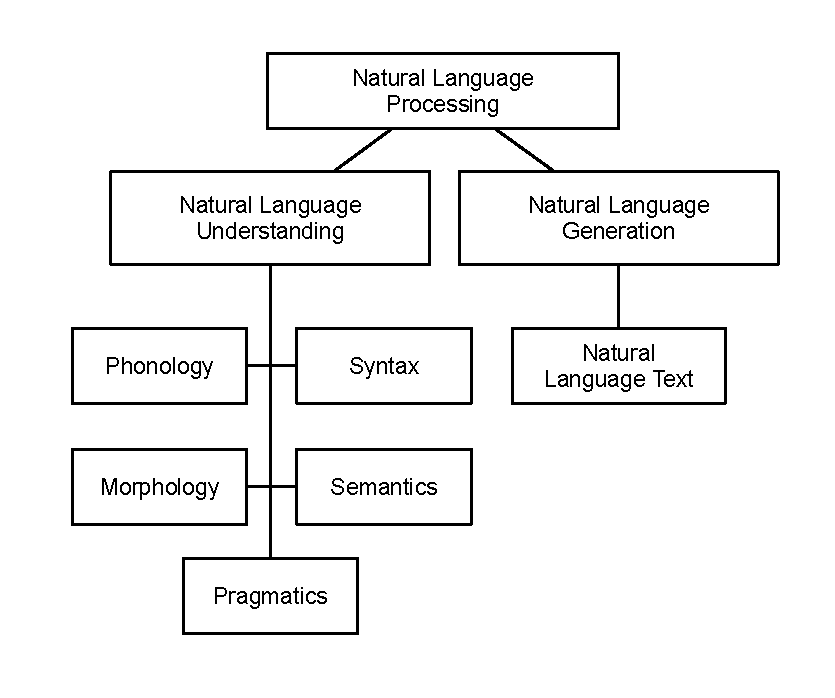
\includegraphics[width=10cm]{./figures/NLP3.eps}
\caption{Classification of NLP}
\label{fig:CNLP}
\end{figure}
Linguistics is the domain in which languages are studied, which involves the meaning of language, and the context language finds itself \cite{Bates9977}. The important terminologies of NLP are: (1) Phonology that refers to the relationship in sound, (2) Morphology word formation, (3) Syntax the sentence structure, (4) Semantics that refers to the arrangement of words and their meaning \cite{hassan2021natural} and (5) Pragmatics which refers to understanding.

To simplify the complexity of Natural Language Processing, it can be broken up into four distinct stages see Figure \ref{fig:stepsnlp}. In a real-world scenario, these stages seldom occur separated. In the overview that follows it is assumed that the syntactic analysis and semantic analysis is done by the pre-processing. The rest of this section contains the processes shown in the figure.
\begin{figure}[htbp]
\centering
\includegraphics[width=10cm]{./figures/NLPstep.eps}
\caption{Steps in Natural Language Processing}
\label{fig:stepsnlp}
\end{figure}
\subsection{Morphological processing}
The first logical step in a typical NLP system is morphological processing. In this step the text will be broken down into sets of tokens corresponding to the equivalent words, sub-words and punctuation forms \cite{Bates9977}. For example, a word like "unnecessarily" can be broken down into three sub-word tokens: un - necessari - ly.

Morphology can be defined as a study of how words can be modified to have similar meanings but used in different syntax. Modifying these words are typically done by adding prefixes and or postfixes. Generally, word modification can be broken down into three components:
\begin{itemize}
    \item Inflection: words can be represented differently based on the syntax they find themselves.
    \item Derivation: new words are made from existing words. Determines, determining, and determined are from the root determine.
    \item Compounding: new words are made by the grouping of existing words. It is not used so much in English (Example "toothpaste") but is widely used in other languages.
\end{itemize}

Outputs from the Morphology phase is a set of tokens. These tokens can contain identifiable data that is needed for the parser to do it's job. The next stage of processing is syntax and semantic analysis.

\subsection{Syntax and Semantic analysis}

A language processor has certain tasks it needs to perform which is syntax analysis and semantic analysis. There are two main aims for syntax analysis: (1) to check if an sentence is well formed, and (2) to break up the structure to show syntactic relationships between the words. A syntactic analyzer (parser) does this by using a dictionary of words (lexicon) and a set of syntax rules (grammar). The usage of a dictionary and syntax rules indicates how syntactic categories can be combined to form phrases of different types \cite{nation2007dissecting,liddy2001natural,feldman1999nlp}.

This syntax-semantic combination could deconstruct the sentence "The large cat chased the rat" as follows:
\begin{figure}[htbp]
\centering
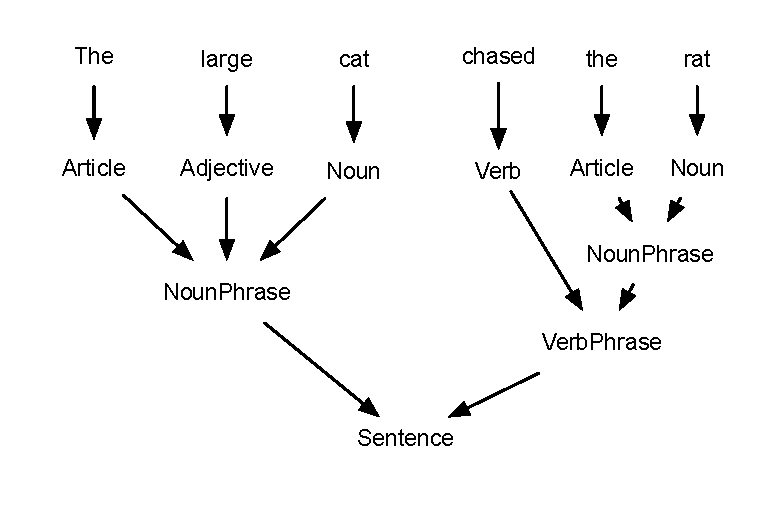
\includegraphics[width=10cm]{./figures/sen.eps}
\caption{Deconstruction of a sentence}
\label{fig:sentence}
\end{figure}
One of the tasks of a language processor is to analyze a sentence and produce a formal notation that concisely expresses the semantics of a sentence and is called Semantic analysis.

When constructing a model, semantic analysis plays the roles of finding meaning of the words in the sentence. In order for that to happen, the dictionary of the model should include weather the words are noun, verb or adjectives. The grammar rule in figure \ref{fig:sentence} with VerbPhrase to Verb, NounPhrase states how the syntactic group is formed.

The important part of this section is to understand that the syntax and semantic analysis phase is of vital importance for any NLP system or tool. The next stage of processing is semantics and pragmatic.
\subsection{Semantics and Pragmatic}

After the combined stages, syntax and semantic analysis, the next stage of processing is pragmatics. There is no clear distinction between semantics and pragmatics \cite{Stern2004}, but for the purpose of this study we make the distinction as follows: semantics studies the meaning of the word and their meaning within sentences whereas pragmatic studies the same word and meaning but within a certain context. Doing semantic analysis on a sentence like "The large cat chased the rat"  can only provide a string of text which translates to the large cat but the identity of the cat. Pragmatic analysis like the example supplied described, simply maps the actual objects which exist in a certain context to a reference obtained during semantic analysis \cite{russell2016artificial}.

This section has provided examples of how analyzing human languages creates certain challenges within the Natural Language Processing domain. In the next section, we will discuss Topic modeling.
\section{Topic modeling} \label{ssec:tmodel}

Language models has recently been used to aid speech recognition and handwriting recognition by showing textual data. Language modeling can be defined as a probability distribution derived from words in an indexed vocabulary \cite{croft2010search}.
\say{They can be used to create new documents by sampling words according to the probability distribution, consider the language model is a pool of words, where the probabilities determine how many occurrences of a word are in the pool, then we can generate word sequences by reaching in, drawing a word, writing it down, putting the word back in the pool and drawing again.} \cite{titov2008modeling}.
This generative process is approximating the model of the topic that the author of the document had in mind when she/he was writing it \cite{raghuveer2012legal}.
A traditional generative model of a language can be used to either recognize patterns of strings or to generate documents \cite{Sajjadi2018AssessingGM}. The generative model as illustrated in figure \ref{fig:automon} as a finite automaton that generates documents.
\begin{figure}[htbp]
\centering
\includegraphics[width=7cm]{./figures/automon8.png}
\caption{A finite automaton and string it generates}
\label{fig:automon}
\end{figure}
Topic modeling has been used as a technique to identify concepts and annotate large text corpora, to keep track of topics over time, and to assess the similarity between topics and  documents. 
The purpose of topic modeling is to analyze data or documents to look for patterns and latent topics. After the topics were identified they would be represented by means of a probability distribution. Topic modeling has been actively applied to several tasks, analysis of scientific patterns  \cite{lau2012line,yi2009comparative,wei2006lda,yi2009comparative}, and scholarly publication search engines \cite{newman2010evaluating}.

Topic modeling is a range of generative models for language that specifies procedures by which documents are built \cite{blei2003latent}. The most preferred algorithm of topic modeling is Latent Dirichlet Allocation (LDA) which describes a generative model for topics and documents \cite{blei2003latent}. 

\subsection{Latent Dirichlet Allocation Algorithm} \label{ssec:LDAA}

Latent Dirichlet Allocation (LDA) is a type of topic model that associates multiple topics for a document. A topic is a distribution over a fixed vocabulary \cite{chaney2012visualizing}. In each topic the distribution of words is different. Assuming the topics are specified before the documents are generated. The documents are generated by the following processes. Initially, the random distribution of topics is selected. For each word in the document a random topic is selected from the distribution of topics. Finally, a word is selected from the topic \cite{blei2003latent,mekonnen2017topic}.

The goal of topic modeling is to discover topics from a collection of documents automatically. To compute the hidden topic structure from documents the probability distribution of the hidden variables given must be computed \cite{mimno2012sparse}.

%\subsection{Use case: Language model and Latent Dirichlet Allocation example}
%To show the process of generating a topic model using the LDA algorithm for a particular document we look at a paper from the ISSA conference corpus. 

%After removing common stop words, we can optionally apply lemmatization or stemming to the corpus. In our example, we only remove stop words since the context of each word or the correct order does not matter. The Bag-of-Words (BOWs) representation will serve as input for our LDA process to generate the LDA model \cite{alghamdi2015survey}.

%In our example, we are using a corpus that consists of 100 papers. This corpus information is needed for smoothing methods that could be applied to the language model. A term not appearing in our paper but in all of the other papers could get a higher probability in the language model than a term appearing in only one paper.

%When applying the LDA algorithm to generate latent topics, we take the BOW representation of all the documents in the corpus. Only the top 10 most likely terms will be displayed. They cover different aspects of Information Security.
\subsection{Topic Model Validation}
The quality, performance and the efficiency of the topic model must be evaluated \cite{ramirez2012topic}. Topic validations have been created to compare the quality of different algorithms. The first approach is to evaluate the topic models based on perplexity, which is calculated on how well the topics were extracted using the training set, and allows to predict the occurrence of words belonging to the training set \cite{ramirez2012topic}.

Other approaches focus on the semantic coherence of the topics. \citeA{chang2009reading} introduced human validation of topical coherence via intrusion tests. The judges had to find the intruder in the evaluated topics and if the intruder was easy detected that means the other words has a strong thematic correlation. However, the process requires manual validation of every build model.
Automatic approaches have been proposed by \citeA{newman2010automatic}, by using Point-wise Mutual Information (PMI) to calculate the co-occurrence in google search results for all given word pairs in the topic. This approach achieved similar results as human coders/judges \cite{alsumait2009topic}.

\subsection{Additional Topic Modeling Tools and Techniques}

Many researchers worked on NLP, building tools and systems which made NLP to what it is today. Tools such as Sentiment analysers, Part of Speech (POS) taggers, Chunking, Name Entity Recognition, Emotion detection and, Topic Modeling. 
A Sentiment analyser works by extracting sentiments about a given topic. Sentiment analysis consists of a topic feature extraction, sentiment extraction and, association by relationship analysis \cite{yi2003sentiment}. Sentiment analysis uses two linguistic resources namely; the sentiment lexicon and the sentiment pattern database \cite{nasukawa2003sentiment}. It analyzes a document for positive and negative words and gives them a rating on a scale of -5 and +5.

Part-of-Speech (POS) tagger can be defined as a piece of software that reads in text and assigns parts of speech to tokens, parts of speech like noun,  verb and adjective. POS tagging is a daunting task because a word can represent more than one speech at different times. Substantially amount of research has been conducted in European languages, and research has shifted to improve POS taggers for other languages like Arabic, Sanskrit \cite{tapaswi2012treebank}, Hindi \cite{ranjan2003part} etc. It can effectively tag and classify words as noun, verb, adjectives, etc. Technological improvements for part of speech tagging can work efficiently on European languages but still lacks advancement on Asian languages \cite{hirschberg2015advances}. The POS tagger used for the Sanskrit language uses the treebank technique \cite{bengoetxea2010application}, Arabic uses the Support Vector Machine (SVM) \cite{diab2004automatic} approach to tokenize, POS tag and annotate phrases in Arabic text.

Chunking is also known as Shadow Parsing, it works by labeling pieces of a sentence with syntactic correlated keywords like Noun phrase and Verb phrase(NP or VP). Each sentence that is being tagged starts with a unique tag marked as Begin chunk (B-NP) tag or Inside chunk (I-NP) tag. Chunking can be evaluated by means of the CoNLL 2000 shared task, which provides test data for chunking \cite{sang2000introduction}. Since the rise of CoNLL 2000 much more systems raised, some reporting around 94.3\% F-Measure score \cite{sha2003shallow,mcdonald2005flexible,sun2008modeling}.

The usage of Named Entity Recognition (NER) in places such as the Internet is problematic because people do not use tradition or academic English \cite{nadeau2007survey}. This brings down the overall performance and quality of language processing tools. By annotating the phrases on unlabeled, in domain and out domain data improves the performance compared to traditional language processing tools \cite{katiyar-cardie-2018-nested}.

Emotion detection is similar to sentiment analysis but used in the social media scene on mixing of two languages (English and one other language). It categorizes statements into 6 different groups based on emotions, namely; sadness, happiness, disgust, fear, surprise, and anger. During the categorizing process, the identification of ambiguous words that are in English + the other language should commence determining the base language of the text. Determining the base language would accelerate the performance and quality of the detection \cite{khurana2017natural}.

Event discovery in social media feeds that uses a graphical model and NER to determine whether it contains the name of a person, city, place, etc. The model operates by listening to noisy data and extracting records and keywords of the events from multiple data streams, despite the noise and the use of irregular language, the model is able to extract records with very high accuracy \cite{benson2011event}. 

\section{Summary}
There has been so much done trying to satisfy the problem of information overload over the past few years that have been using Machine Learning.

In this chapter we discussed why Machine Learning played such a pivotal role in the development in all of these concepts: Document Clustering, Natural Language Processing, and Topic Modeling. 


The next chapter, presents the research methodology that was followed.